\documentclass[aspectratio=169]{beamer}

% --- CONFIGURACIÓN DEL TEMA PROFESIONAL ---
\usetheme{Madrid}
\usecolortheme{default}

% Definición de colores: Paleta "Siena Corporativo"
\definecolor{ProSienna}{RGB}{140,56,35}      % Siena oscuro/Terracota elegante
\definecolor{DarkSienna}{RGB}{90,30,15}      % Siena muy oscuro para contrastes
\definecolor{Charcoal}{RGB}{50,50,50}        % Gris carbón profundo
\definecolor{WarmBeige}{RGB}{245,242,238}    % Blanco cálido/Beige para bloques

% Aplicación de colores a la plantilla
\setbeamercolor{palette primary}{bg=ProSienna,fg=white} 
\setbeamercolor{palette secondary}{bg=Charcoal,fg=white} 
\setbeamercolor{palette tertiary}{bg=DarkSienna,fg=white} 
\setbeamercolor{palette quaternary}{bg=DarkSienna,fg=white}

\setbeamercolor{frametitle}{bg=ProSienna,fg=white} 
\setbeamercolor{title}{bg=ProSienna,fg=white} 
\setbeamercolor{structure}{fg=ProSienna} 
\setbeamercolor{item}{fg=ProSienna} 
\setbeamercolor{normal text}{fg=black,bg=white} 
\setbeamercolor{block title}{bg=ProSienna,fg=white}
\setbeamercolor{block body}{bg=WarmBeige,fg=black}

% --- CONFIGURACIÓN DE LA NAVEGACIÓN SUPERIOR ---
\useoutertheme[subsection=false]{miniframes}
\setbeamercolor{section in head/foot}{fg=white,bg=DarkSienna}
\setbeamercolor{mini frame}{fg=WarmBeige}

\setbeamertemplate{headline}{
  \begin{beamercolorbox}[wd=\paperwidth,ht=5ex,dp=2.5ex]{section in head/foot} 
    \rule{0pt}{0pt} 
    \hfill\insertnavigation{0.9\paperwidth}\hfill 
    \rule{0pt}{0pt}
  \end{beamercolorbox}
}

% --- AUTOMATIZACIÓN DE DIAPOSITIVAS DE SECCIÓN ---
\AtBeginSection[]{
  \begin{frame}[c]
    \vfill
    \makebox[\textwidth][c]{
        \begin{beamercolorbox}[wd=0.8\paperwidth,sep=16pt,center,rounded=true,shadow=true]{title}
          \usebeamerfont{title}\Huge\textbf{\insertsection}
        \end{beamercolorbox}
    }
    \vfill
  \end{frame}
}

% --- PAQUETES BÁSICOS Y JUSTIFICACIÓN ---
\usepackage[utf8]{inputenc}
\usepackage[spanish]{babel}
\usepackage{amsmath}
\usepackage{graphicx} 
\usepackage{ragged2e}       

\addtobeamertemplate{frame begin}{}{\justifying}
\addtobeamertemplate{block begin}{}{\justifying}
\addtobeamertemplate{itemize/enumerate body begin}{}{\justifying}
\addtobeamertemplate{itemize/enumerate subbody begin}{}{\justifying}

% --- INFORMACIÓN DEL TÍTULO ---
\title[StochasticATM]{StochasticATM: Neural SDE y Algoritmos Genéticos}
\subtitle{Modelado Estocástico y Optimización de Rutas Aéreas}
\author[Berredo, Fernández, Rodríguez]{Lucas Berredo, Edgar Fernández, Juan Rodríguez}
\date{14 de abril de 2026}

\begin{document}

% --- DIAPOSITIVA DE TÍTULO ---
\begin{frame}
  \titlepage
\end{frame}

% --- SECCIÓN 0: INTRODUCCIÓN ---
\section{Introducción}

\begin{frame}{Visión General del Proyecto}
  \begin{block}{StochasticATM}
    Proyecto colaborativo enfocado en la aplicación de \textbf{Ecuaciones Diferenciales Estocásticas Neuronales (Neural SDEs)} para la Gestión del Tráfico Aéreo (ATM).
  \end{block}
  \vspace{0.3cm}
  \begin{itemize}
    \item \textbf{Fase actual:} Investigación y prototipado (MVP), sentando las bases algorítmicas para sistemas más robustos.
    \item \textbf{Objetivos principales:}
    \begin{itemize}
        \item Construir una arquitectura reutilizable y escalable para el modelado ATM.
        \item Demostrar la viabilidad del modelado predictivo con \textit{conciencia de incertidumbre} (gráficos de abanico, trayectorias de Monte Carlo).
        \item Garantizar la interoperabilidad total entre los módulos de extracción, predicción y optimización.
    \end{itemize}
  \end{itemize}
\end{frame}

% --- SECCIÓN 1: TRABAJO DE LOS DATOS ---
\section{Trabajo de los Datos}

\begin{frame}{Generación y Extracción de Datos}
  El entrenamiento del modelo depende de una ingesta de datos representativa y de alta calidad.
  \begin{columns}
    \begin{column}{0.47\textwidth}
      \begin{block}{Extracción (OpenSky API)}
        \begin{itemize}
          \item Descarga de trayectorias de llegadas históricas para aeropuertos configurados.
          \item Generación de rutas detalladas por aeronave.
        \end{itemize}
      \end{block}
    \end{column}
    \begin{column}{0.5\textwidth}
      \begin{block}{Ingeniería de Características}
        Cálculo de variables físicas derivadas:
        \begin{itemize}
          \item Velocidad horizontal y tasa vertical.
          \item Estimación de \textbf{flujo de combustible vía OpenAP} (perfil A320).
          \item Consumo acumulado por trayectoria.
        \end{itemize}
      \end{block}
    \end{column}
  \end{columns}
\end{frame}

\begin{frame}{Normalización y Preparación}
  \begin{itemize}
    \item \textbf{Pipeline de Procesamiento:} Preparación y filtrado de las características crudas extraídas de los vuelos históricos.
    \item \textbf{Estabilidad Numérica:} Estandarización minuciosa de las escalas de las variables. Este paso es estrictamente necesario para evitar inestabilidades y explosiones de gradiente durante el entrenamiento de la Neural SDE.
    \item \textbf{Exportación:} Los datos se consolidan y exportan como tensores de PyTorch (\texttt{.pt}), listos para ser introducidos en la red neuronal.
  \end{itemize}
\end{frame}

% --- SECCIÓN 2: MODELO 1 ---
\section{Modelo 1: Neural SDE}

\begin{frame}{Contexto: Del Determinismo a la Estocasticidad}
  La industria ATM actual depende de modelos deterministas (como BADA) que no capturan la naturaleza continua y ruidosa del vuelo.
  \begin{itemize}
    \item \textbf{Limitación de Redes Discretas:} Las RNN o Transformers fallan al adaptarse al continuo físico y a las irregularidades de sensores ADS-B.
    \item \textbf{Propuesta:} Implementar \textbf{Neural SDE} para parametrizar derivadas de estados continuos.
    \item \textbf{Ventaja Clave:} Capacidad de cuantificación de incertidumbre robusta (Robust UQ) y separación de ruido de sensores.
  \end{itemize}
\end{frame}

\begin{frame}{Fundamento Matemático e Implementación}
  El estado latente se controla mediante la ecuación diferencial estocástica basada en el cálculo de Itó:
  \begin{equation}
    dh(t) = f_{\theta}(h(t),t)dt + g_{\phi}(h(t),t)dW(t)
  \end{equation}
  \begin{itemize}
    \item \textbf{$f_{\theta}$ (Red de Deriva):} Componente determinista parametrizado.
    \item \textbf{$g_{\phi}$ (Difusión):} Modula las fluctuaciones del proceso Browniano $dW(t)$.
    \item \textbf{Eficiencia:} Uso del \textbf{Método Adjunto} para un coste de memoria constante $\mathcal{O}(1)$.
  \end{itemize}
\end{frame}

\begin{frame}{Predicción Multivariable Estocástica}
  \begin{columns}
    \begin{column}{0.45\textwidth}
      El modelo predice simultáneamente variables críticas con intervalos de confianza:
      \begin{itemize}
        \item Flujo de combustible y Velocidad (TAS).
        \item Altitud y Tasa Vertical.
        \item Track (Sin/Cos) para orientación.
      \end{itemize}
      \small{Estas inferencias continuas permiten una evaluación precisa de la viabilidad espacial y aerodinámica.}
    \end{column}
    \begin{column}{0.55\textwidth}
      \centering
      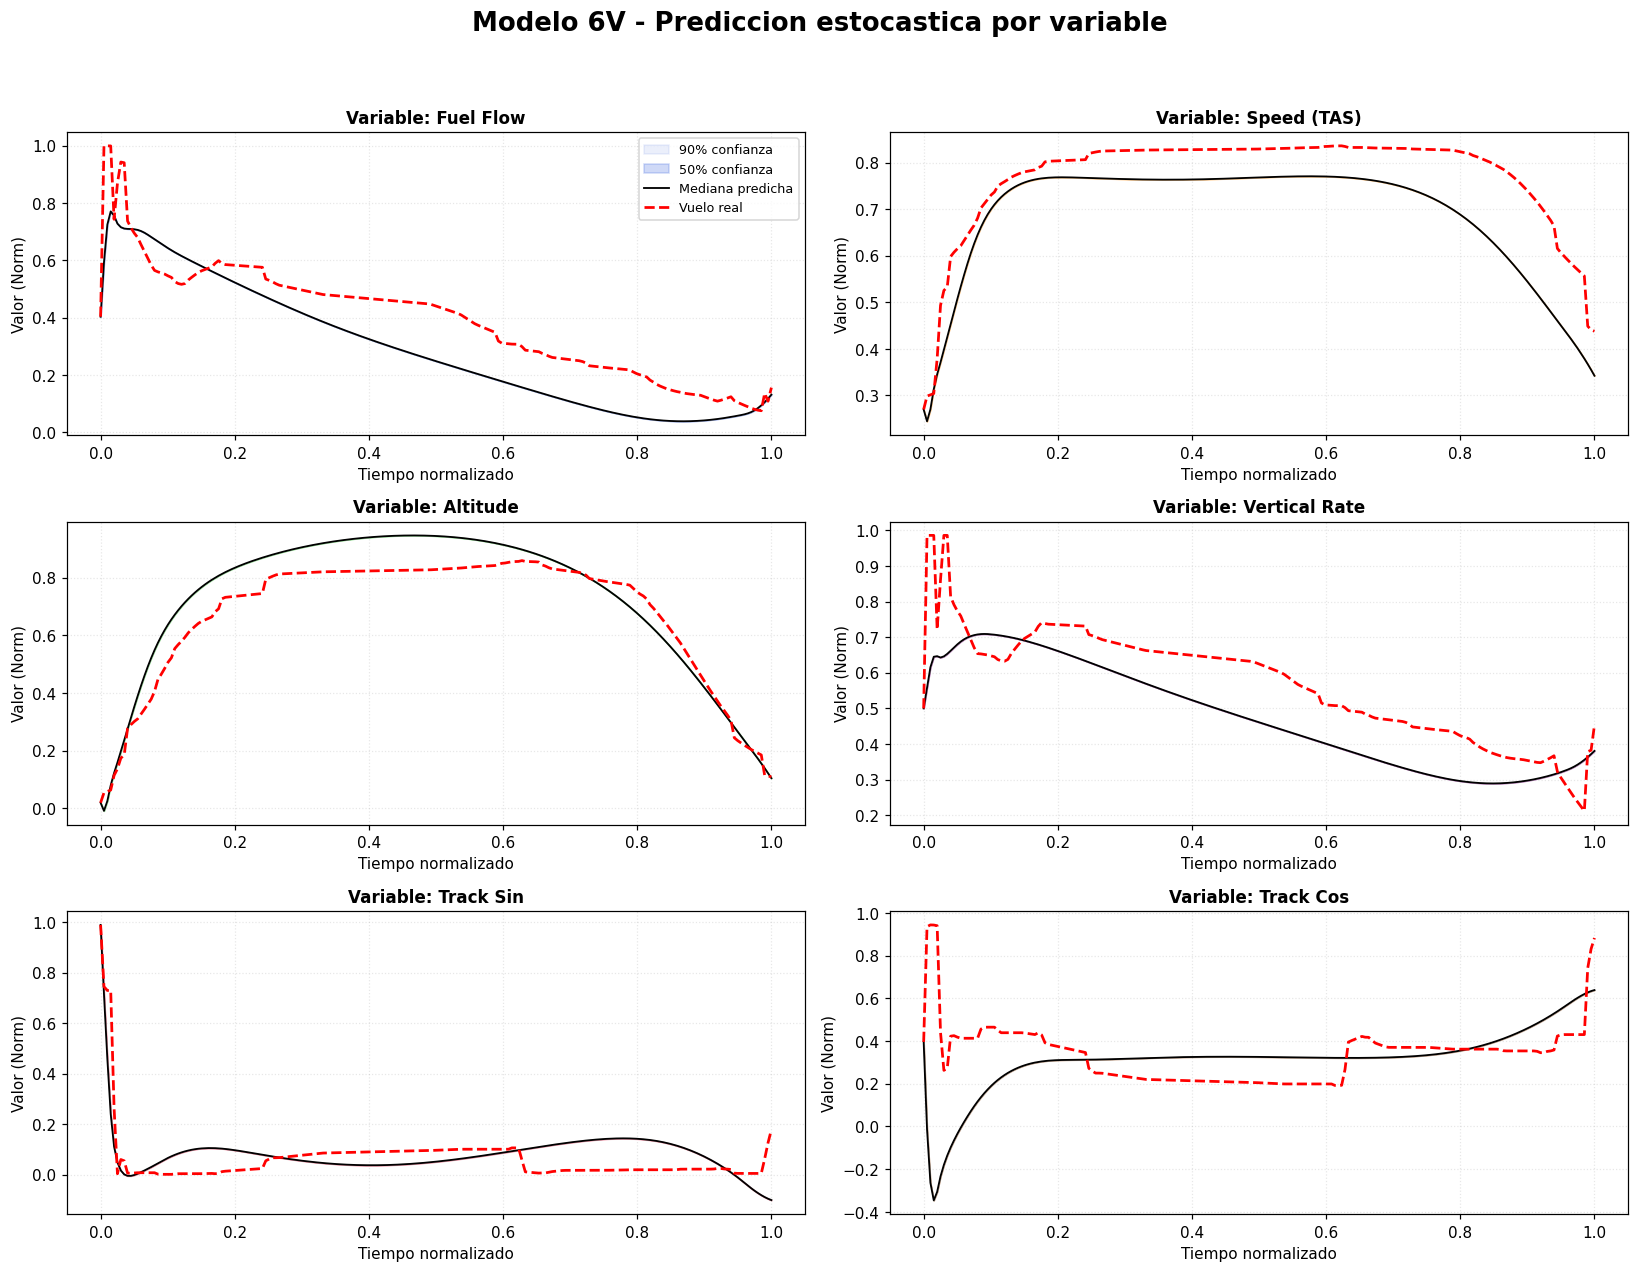
\includegraphics[width=\textwidth]{modelo-6v.png}
      \captionof{figure}{Modelo 6V - Predicción estocástica por variable.}
    \end{column}
  \end{columns}
\end{frame}

% --- SECCIÓN 3: MODELO 2 ---
\section{Modelo 2: Algoritmo Genético}

\begin{frame}{Framework del Algoritmo Genético (AG)}
  Nuestro sistema implementa un AG evolutivo diseñado para navegar un espacio topológico n-dimensional.
  \begin{itemize}
    \item \textbf{Interacción Física:} El AG interactúa continuamente con el motor de física \textit{NeuralFuelSDE}.
    \item \textbf{B-Splines:} En lugar de mallas masivas, usamos puntos de control parametrizados para evitar la explosión combinatoria.
    \item \textbf{Resultado:} Rutas intrínsecamente suaves, navegables y computacionalmente económicas de mutar.
  \end{itemize}
\end{frame}

\begin{frame}{Resolución Dinámica de Nudos y Elitismo}
  \begin{itemize}
    \item \textbf{Filtro de Saneamiento:} El algoritmo "desenreda" bucles proyectando puntos sobre el vector principal y aplicando \texttt{.argsort()}.
    \item \textbf{Elitismo Rígido:} Protegemos las mejores trayectorias frente al ruido browniano de la SDE.
    \item \textbf{Early Stopping:} Evita el gasto computacional innecesario una vez alcanzada la convergencia.
  \end{itemize}
\end{frame}

\begin{frame}{Evasión de Clima: El Puente de Física Exógena}
  \begin{columns}
    \begin{column}{0.5\textwidth}
      \begin{itemize}
        \item \textbf{Lógica de Clima:} La entrada en celdas de tormenta reduce la \textit{velocidad efectiva}.
        \item \textbf{Penalización:} Al volar más lento, el tiempo de integración aumenta, resultando en un \textbf{consumo exponencial}.
        \item El AG aprende a rodear obstáculos para minimizar el coste sin algoritmos de evasión explícitos.
      \end{itemize}
    \end{column}
    \begin{column}{0.5\textwidth}
      \centering
      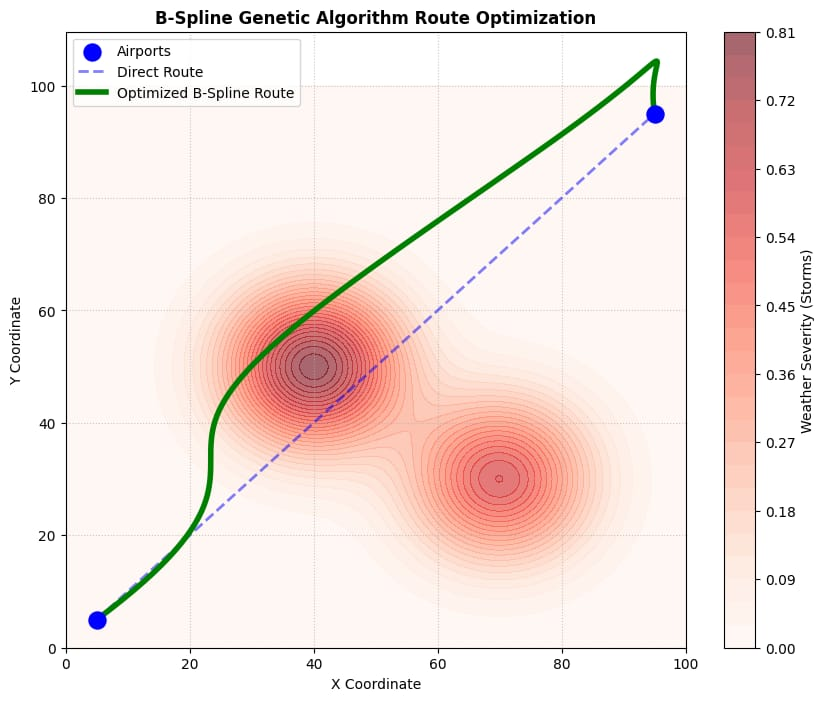
\includegraphics[width=\textwidth]{optimizacion-ruta.jpeg}
      \captionof{figure}{Optimización de ruta evitando meteorología adversa.}
    \end{column}
  \end{columns}
\end{frame}

% --- SECCIÓN 4: APLICACIONES ---
\section{Aplicaciones y Futuro}

\begin{frame}{Casos de Uso Industriales}
  \begin{block}{Adopción en el sector ATM y Aerolíneas}
    \begin{itemize}
      \item \textbf{Optimización de Operaciones:} Reducción directa de la huella de carbono y costes operativos mediante rutas de combustible mínimo.
      \item \textbf{Soporte a la Decisión (ATC):} Herramientas de predicción de conflictos que integran la incertidumbre real del vuelo.
      \item \textbf{Certificación Gubernamental:} La capacidad de separar incertidumbre intrínseca de errores de sensor es un requisito clave para futuras certificaciones de sistemas autónomos.
    \end{itemize}
  \end{block}
  \begin{itemize}
    \item \textbf{Escalabilidad:} El diseño modular permite integrar nuevos sensores (radar, LIDAR) sin cambiar la arquitectura central.
  \end{itemize}
\end{frame}

% --- CONCLUSIÓN ---
\section{Conclusión}

\begin{frame}{Hitos y Futuro}
  \begin{itemize}
    \item \textbf{Éxito del MVP:} Framework transversal para extracción, predicción y ahorro de combustible.
    \item \textbf{Innovación:} Unión de Neural SDE y Algoritmos Genéticos para cuantificación probabilística del error.
    \item \textbf{Próximos Pasos:} Implementación de métodos más costosos para optimizar la convergencia incondicional y el despliegue en entornos de mayor escala.
  \end{itemize}
  \begin{center}
    \vspace{0.5cm}
    \small{Repositorio y documentación disponibles en: \\ \url{https://github.com/LucasBerredo/StochasticATM}}
  \end{center}
\end{frame}

\end{document}